\newpage
\section{Zielsetzung}
    Das Ziel des Versuches ist die Untersuchung des Röntgenemissionsspektrums  von Kupfer der
    Röntgenabsorbtionsspektren anderer Materialien.\\ Des Weiteren sollen die maximale Intensität der Röntgenröhre und das energetische Auflösevermögen der Apparatur bestimmt werden.
    Zusätzlich wird auch das Moseleysche-Gesetz überprüft.

\section{Theoretische Grundlagen }

\subsection{Erzeugung von Röntgenstrahlung}

Röntgenstrahlung ist jene Strahlung, welche Energien von $\SI{10}{\eV}$ bis $\SI{200}{\kilo\eV}$ besitzt.\\
Eine der vielen Methoden um Röntgenstrahlung zu Erzeugen ist die Beschleunigung von, durch den glühelekktrischen Effekt ausgelösten, Elektronen auf eine Bremsanode.\\
Dabei entsteht zum einen das kontinuierliche Bremsspektrum und das  von dem Anodenmaterial abhängige charakteristische Spektrum.\\
\begin{wrapfigure}{r}{5cm}
    \centering
    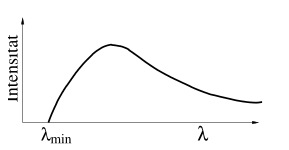
\includegraphics[width=6cm]{latex/images/kurve1.PNG}
    \caption{Eine schematische Darstellung der Intensität des kontinuierlichen Spektrums der Bremsstrahlung\protect \cite{V602}.}
    \label{img:comp}
\end{wrapfigure}

\noindent
Das kontinuierliche Spektrum entsteht, wenn Elektronen beim Eintreten in die Anode vom Coulomb-Feld der gebundenen Elektronen abgebremst werden. 
Dabei sendet das abgebremste Elektron Bremsstrahlung aus, welche energetisch der verlorenen kinetischen Energie entspricht.\\
Da die Energie allerdings keinen bestimmten Wert haben muss entsteht ein kontinuierliches Spektrum. Dieses ist in Abbildung \ref{img:kont} qualitativ dargestellt.\\
Die bei diesem Vorgang maximal abgestrahlte Energie ist die komplette kinetische Energie.\\
Da die die Energie des beschleunigten Elektrons $E_{kin}= U \cdot \symup{e_0}$ entspricht, wobei $U$ die angelegte Spannung und $\symup{e_0}$ die Elementarladung \cite{e0} ist, und
$E= \symup{h} \nu$ die Energie des Photons, mit dem Planckschen Wirkungsquantum\cite{h} und der Frequenz ist, ergibt sich für die minimale Wellenlänge:
\begin{equation*}
    \lambda_{min}=\frac{\symup{h \cdot c}}{\symup{e_0}\cdot U}
\end{equation*}
\newline
\noindent
Beim charakteristischen Spektrum wird ein Elektron des Anodenmaterials durch einen Stoß angeregegt und hinterlässt so eine Leerstelle in einer der inneren Schalen. 
Beim Zurückfallen auf die innere Schale wird dann die Differenz der Energieniveaus $\symup{h} \cdot \nu=  E_M-E_N$ als Photon abgestrahlt.\\
Da die Energien der Energieniveaus vom Material abhängig sind, sind die gemessenen Linien dieses Prozesses charakteristisch für das Anodenmaterial.\\
Diese Linien tragen Bezeichnungen wie $K_\alpha$, $K_\beta$ oder $L_\alpha$. Der Buchstabe bezieht sich dabei auf die Schalen, auf die die Elektronen zurückfallen. \\
Der griechische Buchstabe im Index repräsentiert dabei den Herkunftsort des Elektrons.\\\\
Die Energie der Niveaus auf den Schalen nimmt ab, je weiter die Schalen vom Kern enfernt liegen. 
Dies liegt daran, dass die innen liegenden Elektronen das Coulomb Potential abschirmen und somit schwächen.\\
Für die Bindungsenergie auf der n-ten Schale $E_N$ gilt dabei:
\begin{equation*}
    E_N=-R_{\infty} z_{eff}^2 \cdot \frac{1}{n^2}
\end{equation*}
Dabei wird auch der Abschirmeffekt der effektiven Kernladung $z_{eff}=z-\sigma$, mit der Kernladungszahl $z$ und der Abschirmkonstante $\sigma$, berücksichtigt.
Des Weiteren ist $R_\infty$ die Rydbergenergie\cite{Ryd}.\\\\

\noindent Da die Elektronen auf den äußeren Bahnen, aufgrund ihres Spins und Bahndrehimpulses, nicht immer die selben Energien besitzen, fransen die zuvor beschriebenen Linien etwas aus.\\
Beim Zurückfallen in ein niedriegeres Energieniveaus variiert die Ausgangsenergie dabei leicht, was zu nah beeinander liegenden Linien führt.\\
Dies nennt sich Feinstruktur, ist aber im folgenden Versuch nicht auflösbar.\\
\begin{wrapfigure}{r}{6cm}
    \centering
    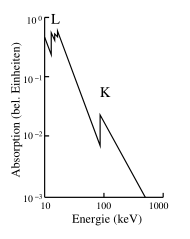
\includegraphics[width=5cm]{latex/images/absorption.PNG}
    \caption{Eine schematische Darstellung der Absorption von Elektronen in Abhängigkeit von deren Energie. Zusätzlich auch noch die K- und L-Kante\protect \cite{V602}.}
    \label{img:comp}
\end{wrapfigure}
Für Energien kleiner als $\SI{1}{\mega\eV}$ sind der Photo- und der Comptoneffekt dominant, was die Absorption und damit den Absorptionskoeffizienten angeht.\\
Dieser sinkt nämlich kontinuierlich bis die Bindungsenergie eines Elektrons in der nächst inneren Schale überschritten wird und sie dann schlagartig steigt.\\
Dies passiert über den Photoeffekt, mit dessen Hilfe das Elektronen herausgelöst wird.\\ 
Diese so entstehenden Kanten werden abhängig von der Ausgangsschale L- oder K-Kante genannt. Dabei gibt es aufgrund der Feinstruktur die Kanten $\symup{L}_{I}$ bis $\symup{L}_{III}$, allerdings nur eine K-Kante.\\
Unter berücksichtigung der Feinstruktur lässt sich die Bindungsenergie der Elektron $E_{n,j}$ übder die Sommerfeldsche Feinstrukturformel bestimmen:
\begin{equation*}
    E_{n,j}= -R_\infty \left( z_{eff,1}^2 \frac{1}{n^2}+ \alpha^2   z_{eff,2}\frac{1}{n^3} \left( \frac{1}{j+ \frac{1}{2}} + \frac{3}{4n}   \right)   \right)
\end{equation*}
Dabei sind, zusätzlich zu den zuvor benannten Variablen, $\alpha$ die Sommerfeldsche Feinstrukturkonstante \cite{sommer}, $n$ die Hauptquantenzahl und $j$ der Gesamtdrehimpuls des Elektrons.\\


SOLL DEFINITION VON SIGMA REIN?


\subsection{Bragg'sche Reflexion}

\begin{wrapfigure}{r}{6cm}
    \centering
    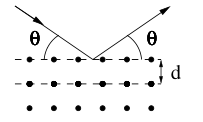
\includegraphics[width=6cm]{latex/images/bragg.PNG}
    \caption{Eine schematische Darstellung der Reflexion eines Photons an polykristalliner Materie\protect \cite{V602}.}
    \label{img:comp}
\end{wrapfigure}
Mit Hilfe von Bragg'scher Reflexion kann die Wellenlänge $\lambda$  und damit auch die Energie bestimmen.
Dafür wird das Licht auf ein dreidimensionales Gitter, wie einen LiF-Kristall gelenkt. Das Licht wird dabei an der oberen und an den tiefer liegenden Gitterebenen reflektiert.\\
Für einen Glanzwinkel $\theta$, bei dem der Wegunterschied des Lichtes $n\pi$ beträgt, entsteht konstruktive Interferenz.\\
Daraus lässt sich dann über die so gennante Bragg'sche Bedingung die Wellenlänge bestimmen:
\begin{equation*}
    2 d \sin \theta =n \lambda
\end{equation*}
Dabei ist d die Gitterkonstante, welche für einen LiF-Kristall $d_{LiF}=\SI{201.4}{\pico\metre}$ entspricht, und $n$ die Beugungsordung.



